\chapter{Participação na RoboCup 2017}\label{cap:robocup_2017}

Uma segunda versão do \textit{firmware} abstraído em \textit{hardware} foi desenvolvida para a Robocup 2017, realizada em Nagoya, Japão, no final de julho de  2017. Os robôs, com novo \textit{firmware} e novas placas de circuito impresso, funcionaram como pretendido, sendo capazes de receber as informações da inteligência e executar os comandos, permitindo atingir o 16º lugar, jogando 6 partidas, das quais venceu 2.
Entretanto, o projeto continuará evoluindo, pois aprimoramentos precisam ser feitos, por exemplo, na malha de controle. Também pensa-se em trocar os motores DC por motores \textit{brushless}. Fazer tais alterações será mais fácil, graças ao caráter modular do projeto.

\begin{figure}
	\centering
	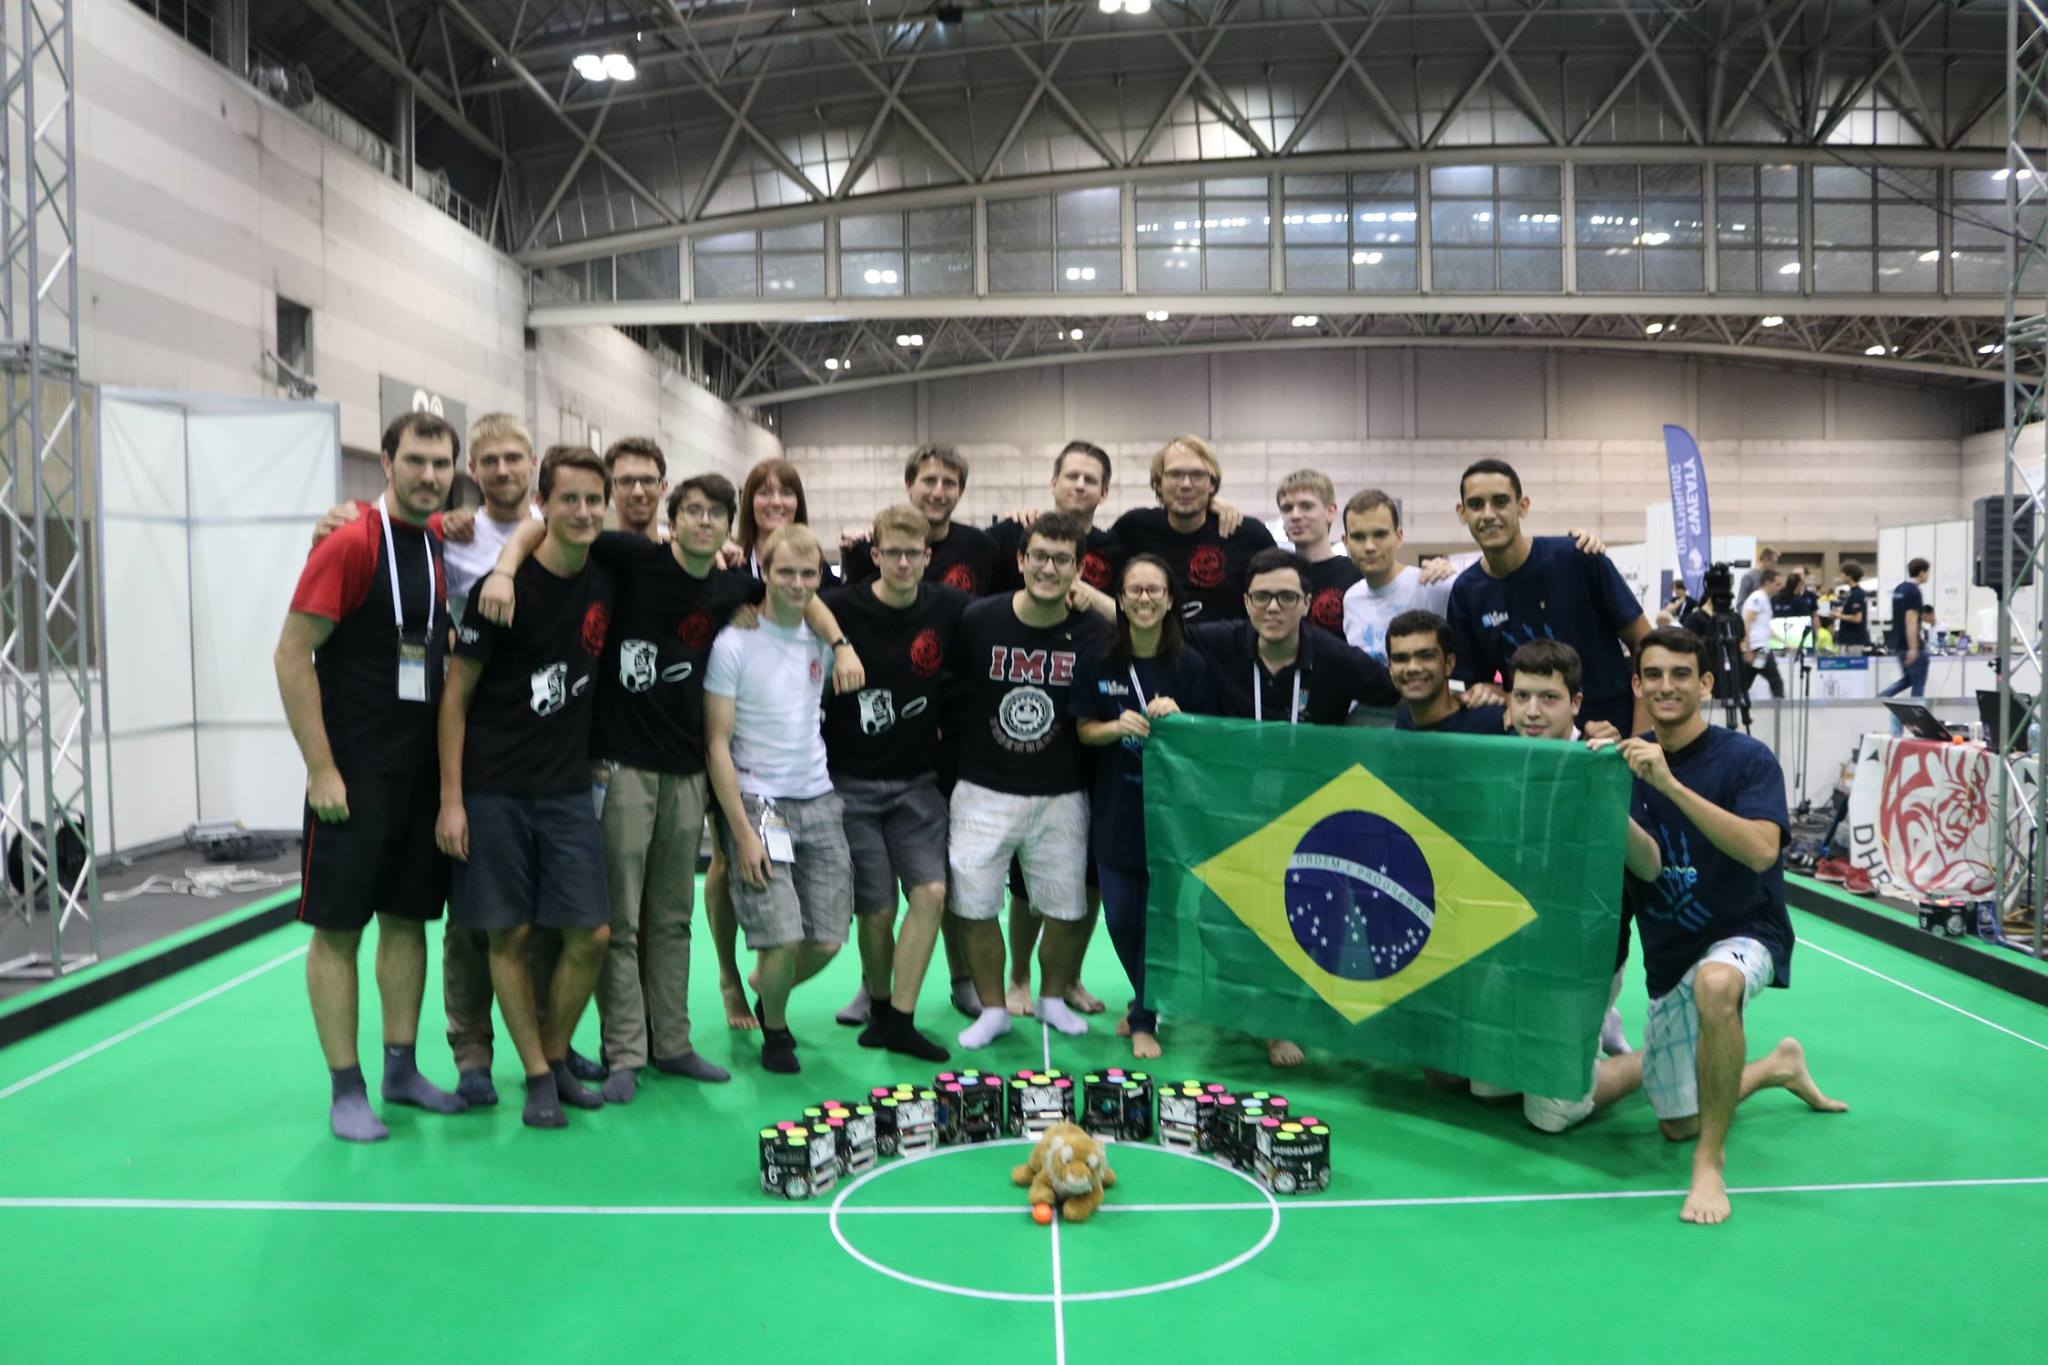
\includegraphics[scale=0.22]{robocup2017}
	\caption{RoboIME e equipe adversária após uma partida}
	\label{fig:robocup_2017}
\end{figure}

% Ramificação constante ou taxa constante

% vim: tw=80 et ts=2 sw=2 sts=2 ft=tex spelllang=pt_br,en

